%%%%%%%% ICML 2023 EXAMPLE LATEX SUBMISSION FILE %%%%%%%%%%%%%%%%%

\documentclass{article}

% Recommended, but optional, packages for figures and better typesetting:
\usepackage{microtype}
\usepackage{graphicx}
\usepackage{subfigure}
\usepackage{booktabs} % for professional tables
\usepackage{float}
\usepackage{caption}
\usepackage{captcont}


\usepackage{tikz}
% Corporate Design of the University of Tübingen
% Primary Colors
\definecolor{TUred}{RGB}{165,30,55}
\definecolor{TUgold}{RGB}{180,160,105}
\definecolor{TUdark}{RGB}{50,65,75}
\definecolor{TUgray}{RGB}{175,179,183}

% Secondary Colors
\definecolor{TUdarkblue}{RGB}{65,90,140}
\definecolor{TUblue}{RGB}{0,105,170}
\definecolor{TUlightblue}{RGB}{80,170,200}
\definecolor{TUlightgreen}{RGB}{130,185,160}
\definecolor{TUgreen}{RGB}{125,165,75}
\definecolor{TUdarkgreen}{RGB}{50,110,30}
\definecolor{TUocre}{RGB}{200,80,60}
\definecolor{TUviolet}{RGB}{175,110,150}
\definecolor{TUmauve}{RGB}{180,160,150}
\definecolor{TUbeige}{RGB}{215,180,105}
\definecolor{TUorange}{RGB}{210,150,0}
\definecolor{TUbrown}{RGB}{145,105,70}

% hyperref makes hyperlinks in the resulting PDF.
% If your build breaks (sometimes temporarily if a hyperlink spans a page)
% please comment out the following usepackage line and replace
% \usepackage{icml2023} with \usepackage[nohyperref]{icml2023} above.
\usepackage{hyperref}
\usepackage{xurl}



% Attempt to make hyperref and algorithmic work together better:
\newcommand{\theHalgorithm}{\arabic{algorithm}}

\usepackage[accepted]{icml2023}

% For theorems and such
\usepackage{amsmath}
\usepackage{amssymb}
\usepackage{mathtools}
\usepackage{amsthm}

% if you use cleveref..
\usepackage[capitalize,noabbrev]{cleveref}

%%%%%%%%%%%%%%%%%%%%%%%%%%%%%%%%
% THEOREMS
%%%%%%%%%%%%%%%%%%%%%%%%%%%%%%%%
\theoremstyle{plain}
\newtheorem{theorem}{Theorem}[section]
\newtheorem{proposition}[theorem]{Proposition}
\newtheorem{lemma}[theorem]{Lemma}
\newtheorem{corollary}[theorem]{Corollary}
\theoremstyle{definition}
\newtheorem{definition}[theorem]{Definition}
\newtheorem{assumption}[theorem]{Assumption}
\theoremstyle{remark}
\newtheorem{remark}[theorem]{Remark}

% Todonotes is useful during development; simply uncomment the next line
%    and comment out the line below the next line to turn off comments
%\usepackage[disable,textsize=tiny]{todonotes}
\usepackage[textsize=tiny]{todonotes}


% The \icmltitle you define below is probably too long as a header.
% Therefore, a short form for the running title is supplied here:
\icmltitlerunning{Project Report Template for Data Literacy 2023/24}

\makeatletter
\newcommand{\showfontsize}{\f@size pt}
\makeatother

\newcommand{\showfont}{\fontname\font}

\begin{document}

\twocolumn[
\icmltitle{Altitude Attitudes: Analyzing Demographic Effects in Flying Etiquette}

% It is OKAY to include author information, even for blind
% submissions: the style file will automatically remove it for you
% unless you've provided the [accepted] option to the icml2023
% package.

% List of affiliations: The first argument should be a (short)
% identifier you will use later to specify author affiliations
% Academic affiliations should list Department, University, City, Region, Country
% Industry affiliations should list Company, City, Region, Country

% You can specify symbols, otherwise they are numbered in order.
% Ideally, you should not use this facility. Affiliations will be numbered
% in order of appearance and this is the preferred way.
\icmlsetsymbol{equal}{*}

\begin{icmlauthorlist}
\icmlauthor{Xinqiao Yang}{equal,first}
\icmlauthor{Kevin Hoffmann}{equal,second}
\icmlauthor{Muhammed \"{O}mer Akgeyik}{equal,third}
\icmlauthor{Moritz L\"{o}nker}{equal,fourth}
\end{icmlauthorlist}

% fill in your matrikelnummer, email address, degree, for each group member
\icmlaffiliation{first}{Matrikelnummer 6003777, xinqiao.yang@student.uni-tuebingen.de, MSc Quantitative Data Science Method}
\icmlaffiliation{second}{Matrikelnummer 6126885, kevin.hoffmann@student.uni-tuebingen.de, BSc Computer Science}
\icmlaffiliation{third}{Matrikelnummer 6042277, muhammed-
oemer.akgeyik@student.uni-tuebingen.de, BSc Computer
Science}
\icmlaffiliation{fourth}{Matrikelnummer 6795289, moritz.loenker@student.uni-tuebingen.de, MSc Cognitive Science}

% You may provide any keywords that you
% find helpful for describing your paper; these are used to populate
% the "keywords" metadata in the PDF but will not be shown in the document
\icmlkeywords{Machine Learning, ICML}

\vskip 0.3in
]

% this must go after the closing bracket ] following \twocolumn[ ...

% This command actually creates the footnote in the first column
% listing the affiliations and the copyright notice.
% The command takes one argument, which is text to display at the start of the footnote.
% The \icmlEqualContribution command is standard text for equal contribution.
% Remove it (just {}) if you do not need this facility.

%\printAffiliationsAndNotice{}  % leave blank if no need to mention equal contribution
\printAffiliationsAndNotice{\icmlEqualContribution} % otherwise use the standard text.

\begin{abstract}
In this project, we aim to analyze airplane etiquette using a dataset collected from a FiveThirtyEight online survey with 1,040 participants. \href{https://github.com/fivethirtyeight/data/blob/master/flying-etiquette-survey/flying-etiquette.csv}{The dataset} includes information on travel habits, seating preferences, and passenger perception.
We discovered this dataset through online platforms and found it helpful in understanding social norms during air travel. It also seems to be of reasonable quality and makes for a fun project.
Our analysis will involve correlations between demographic factors and etiquette opinions to provide insights into passenger interactions. We hope to reveal patterns that can inform discussions on future airline policies and reveal something about human nature. 

\end{abstract}

\section{Introduction}\label{sec:intro}

As more people take to the skies for travel, whether they're seasoned flyers or first-timers, flying has become a common part of modern life. But even with so many people flying, there are still some persistent issues with how people behave during flights. Things like seat reclining, noisy kids, and people using their gadgets have always been problems, and finding practical solutions has been a bit tricky. In this paper, we'll look at three behavior patterns related to demographics that could help us understand and tackle some of these challenges. In the next sections, we'll explain the data we used and why we tested certain ideas, and then we'll share what we found and some thoughts on the limitations of our study. This paper delves into an exploration of three distinct behavioral patterns that interconnect demographic variables with specific etiquette predicaments, offering insightful proposals to mitigate these challenges. \Cref{sec:methods} provides a detailed overview of the dataset and the meticulous data cleaning process, accompanied by an explanation of the rationale behind our hypothesis testing. In \Cref{sec:results}, we unveil the significance of all three hypotheses. \Cref{sec:conclusion} delves into the underlying intuitions behind these hypotheses, shedding light on the inevitable limitations of our analysis, such as the inherent challenge of "response bias." Through this examination, we aim to contribute to a deeper understanding of the intricate interplay between demographic factors and flying etiquette, ultimately enhancing the air travel experience for all.

\section{Data and Methods}\label{sec:methods}

The data was collected through a self-reporting online survey on an American website with 1,040 participants, however, there were only 687 participants who answered all questions. There were two types of questions in the survey: flight-etiquette related questions and demographic questions. Flight-etiquette related questions included travel habits, flight rules following status, reclining seat frequency, and opinion, sense of obligation, rudeness perception, and arm rest usage opinion, while the demographic questions included gender, age, height, household income, education, location, and parenthood state. All participants were US-Americans. Height was measured in inches and is interpreted as a continuous value in our analysis. The answers to all other questions are categorical. 

\begin{figure*}[]
    \includegraphics[width=\textwidth]{bar_overview.pdf}
    \caption{Dataset}
    \label{bar_overview}
\end{figure*}

The data preprocessing involved two parts: First, Data encoding and feature transformation, meaning that we introduced some ordinal structure to some questions according to frequency/extent, and nominal structure to some other questions according to different names of entities, then we transformed the textual data into numerical data, which is more convenient for correlation test and further analysis. With the feature transformation, for the European reader we converted the height from inches into centimeters, making the data more intuitive. Detailed encoding rules are shown in the data preprocessing part in GitHub repository \href{https://github.com/mloenker/flying-etiquette-data-lit}{link}. Second, missing value manipulation, meaning that we made two versions of the completed dataset, one with deleting all rows with at least 1 missing value and another with imputation of missing values. Since the missing value deletion will lead to roughly 34\% data size loss. However, imputation via mode, and other techniques like regression-based imputation can also introduce bias into the dataset.

Next, we did some exploratory analysis to reduce the dimensionality of the features, we conducted Multiple correspondence analysis (MCA) \citep{abdi2007multiple}, which is the categorical version of principal component analysis. However, MCA did not produce satisfactory results with single digit numbers for the explained variance, as the covariance in the dataset was not high enough. Because of this, we stopped pursuing an analysis of the whole dataset and focused on five distinct questions, used to test three hypotheses. To maximize the amount of data samples, we only delete the entries from each specific questions in which the subjects did not provide an answer. This means we have different sample numbers for different questions. For our hypotheses, we did two Chi-squared tests \citep{Pearson1900} and one Analysis of Variance (ANOVA) \citep{anova}.

In Figure \ref{bar_overview}, we showed the six questions which are related to our hypotheses, since it helps in giving an overview of the distribution of different groups in the questions and helps in checking the assumptions of Chi-squared test and ANOVA. We can see height is asymptotically normal distributed, which satisfies the normality assumption of the ANOVA. 

We have also tested the variances of the subgroups of whom answering "yes" and "no" towards the question "Given the opportunity, would you eliminate the possibility of reclining seats on planes entirely", thus, it satisfied the homogeneity assumption of ANOVA in our third hypothesis testing.

Comparing to the case study \citep{relatedwork} on this dataset which solely visualized the percentage of "rudeness" perception of some questions, our project took a deeper look at the correlations of certain features of the flight etiquette, including "Electronics Usage", "Children Bringing" and "Seat Reclining", and we tried to explain what are the potential problems under the intuitive correlation, and what can we suggest for future airline policies.


% This is the template for a figure from the original ICML submission pack. In lecture 10 we will discuss plotting in detail.
% Refer to this lecture on how to include figures in this text.
% 
% \begin{figure}[ht]
% \vskip 0.2in
% \begin{center}
% \centerline{\includegraphics[width=\columnwidth]{icml_numpapers}}
% \caption{Historical locations and number of accepted papers for International
% Machine Learning Conferences (ICML 1993 -- ICML 2008) and International
% Workshops on Machine Learning (ML 1988 -- ML 1992). At the time this figure was
% produced, the number of accepted papers for ICML 2008 was unknown and instead
% estimated.}
% \label{icml-historical}
% \end{center}
% \vskip -0.2in
% \end{figure}

\section{Results}\label{sec:results}
Overall, we took a look at three distinct hypotheses that all center around the etiquette of human behavior on airplanes. We employ a combination of statistical tests and contingency plots to best illustrate the data. For each hypothesis, our approach is first to try to show a significant relationship between the variables and then visualize the direction and type of the relation using the contingency plots. For hypotheses 1 and 2, our preconceived intuitions were confirmed, while the results for our last hypothesis are counterintuitive and maybe even offer a rare window into the psyche of airplane travelers. We used Chi-squared tests for the first two hypotheses, and for both tests we found a sufficient expected frequency of above five. To account for multiple comparisons, we employed a Holm-Bonferroni correction to correct a probable inflated type I error \citep{holm-bonferroni}. However, it has to be noted that the procedure had no impact on significance.

\subsection{Hypothesis 1: Electronics and Age}

First we tested for a relationship between electronics during take-off and age with a total sample size of 843. In the survey, age was divided into four distinct categories, visible in Figure \ref{bar_overview}. All participants are divided roughly equally among the categories. Electronics usage was inquired with the question "Have you ever used personal electronics during takeoff/landing against a flight attendant's instructions?". To test the null hypothesis of no relationship, we used a Chi-squared test. According to the result, we reject the null hypothesis with a p-value of 4.54e-10 after the Holm-Bonferroni correction. We thus find a significant relationship between age and electronics use during take-off. The conditional probabilities we computed also reflect our result of the Chi-squared test, as in Figure \ref{hypothesis1} a notable growth in the magnitude of the red bar becomes evident with advancing age categories.
\begin{figure}[h]
    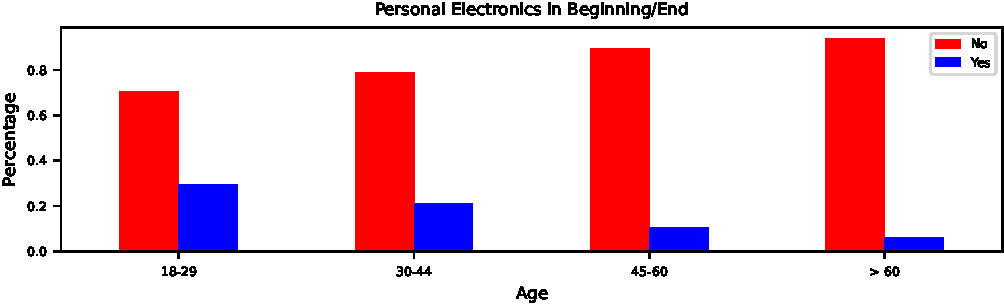
\includegraphics[width=\columnwidth]{hypo_1.pdf}
    \caption{Plot for Hypothesis 1}
    \label{hypothesis1}
\end{figure}


\subsection{Hypothesis 2: Having Children and Finding it rude to bring children}
We next investigated a possible relationship between the question "Do you have any children under 18?" and "In general, is it rude to knowingly bring unruly children on a plane?" with a total sample size of 845. Again, we used a Chi-square test and, according to the result, rejected the null hypothesis of no relationship with a p-value of 2.29e-09 after Holm-Bonferroni correction. Figure \ref{hypothesis2} shows this significant relationship between the categories.  While most people who do not have children think it is rude to bring unruly children on a plane, the fewest people with children under 18 answered the same question with "Yes" represented by the blue bar. There is also a drastic increase in the purple bar when comparing people with and without children under 18. This suggests a substantial difference in the perspectives of people with children under 18 and without, underscoring the potential impact of familial status.
\begin{figure}[h]
    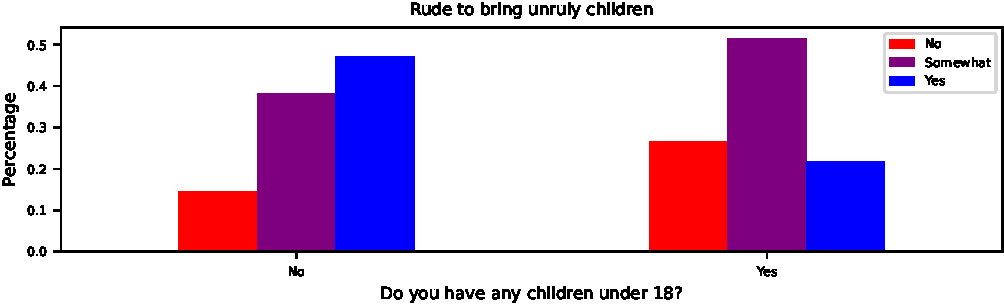
\includegraphics[width=\columnwidth]{hypo_2.pdf}
    \caption{Plot for Hypothesis 2}
    \label{hypothesis2}
\end{figure}


\subsection{Hypothesis 3: Height and the opportunity to eliminate the possibility of reclining seats}
For the last hypothesis, we wanted to investigate a possible relationship between height and the opportunity to eliminate the possibility of reclining seats with a total sample size of 854. Not enough leg space is a common complaint on airlines, and tall people are affected more, so these people may have a bad opinion on seat reclining. We tested for a relationship between height and the question, "Given the opportunity, would you eliminate the possibility of reclining seats on planes entirely?" where we found a significant relationship. For this hypothesis, we used ANOVA. The results were a statistically significant F-value of 5.69 with a corresponding p-value of 0.017 after the Holm-Bonferroni correction. As we examined the mean height for each category of the reclining seats preference, we observed that individuals who would eliminate the possibility of reclining seats on planes entirely have a higher mean height (172.61 cm) compared to those who would not eliminate this option (with a mean height of 170.84 cm). This significance is also visible in \ref{hypothesis3} as an observable upward trend in the blue line is notable with increasing height.
\begin{figure}[h]
    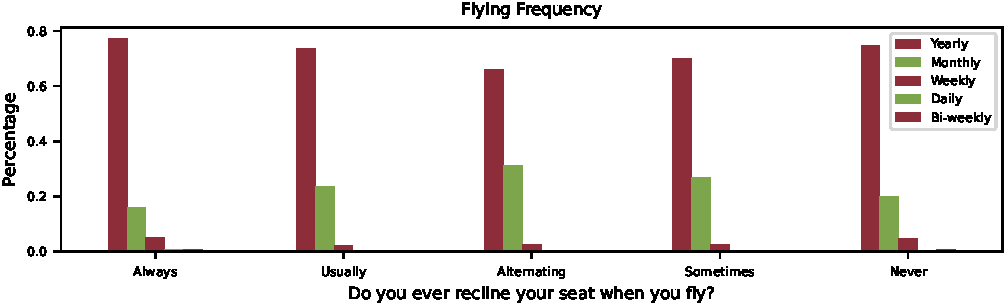
\includegraphics[width=\columnwidth]{hypo_3.pdf}
    \caption{Plot for Hypotheses 3}
    \label{hypothesis3}
\end{figure}



\section{Discussion \& Conclusion}\label{sec:conclusion}

%Use this section to briefly summarize the entire text. Highlight limitations and problems, but also make clear statements where they are possible and supported by the analysis. 
\subsection{Discussion}
Our tests broadly confirmed our preconceived hypotheses. We found a significant relationship between age and electronics use, and the bars in \ref{hypothesis1} show that young people are more likely to use electronics during take-off. We cannot know whether this is due to young people generally using more electronics or due to young people being more likely to disregard rules. We see that the percentage of electronics use shrinks with each age category, so there is not only a difference between young and old but also between all categories. This seems to support the idea that general electronics use is the main driver behind the relationship. 

For our second hypothesis, we found a significant relationship between having children and the attitude towards unruly children on planes. Figure \ref{hypothesis2} shows that people with children were more likely to find bringing unruly children not rude or only somewhat rude compared to people without children. The interesting bit is that the question explicitly only mentions unruly children and not children in general. So we hypothesize that people with children either think their own children are unruly and don't want to call themselves rude or are, in general, less annoyed by unruly children. It could also be the case that they are more aware that children can become unruly in unbecoming situations. Ultimately, we cannot know the exact cause of this relationship. 

In the third hypothesis, we found a significant relationship between height and wanting to eliminate the opportunity to recline seats entirely. It is common knowledge that taller people suffer more from less leg space, and Figure \ref{hypothesis3} shows that this also translates into political demands that affect not only themselves, but all people. Not being able to recline seats would make it harder to sleep on planes, but for some people, this seems to be worth it. Maybe it is a good idea to ask the height in the ticket order system and assign seats with the rule of combining tall and comparatively short people in the same column when they did not have a seat preference. Even if they would have a specific seat preference, the system can still show a recommendation of the seats based on the optimization algorithm.

\subsection{Limitations}
Any data analysis technique will likely exhibit some limitations. First of all, given the nature of self-reporting surveys, respondents may provide socially desirable or biased responses. Issues related to air travel etiquette violating flight attendant instructions, might be underreported or inaccurately reported due to the potential legal consequences associated with such behaviors.

Secondly, the dataset includes missing values for some participants. Particularly in the demographic and etiquette-related questions, some are not answered by everyone. The approach to handle the missing values introduces potential bias and variability in the analyses, which affects the robustness of the results. There is also a limited geographical representation, as all participants in the dataset are U.S. Americans. 

Besides, the variables "Age," and "In general, is it rude to knowingly bring unruly children on a plane?" exhibit a natural ordering of categories, which we didn't use in our analysis techniques. Instead, every category was seen as having the same distance from every other category. Thus, we cannot fully exclude the possibility that stronger statements could be drawn from the data.


Thirdly, for the first hypothesis, one assumption of the Chi-squared test might not be satisfied: Age is distributed almost equally over 4 subgroups, around 25.05\% on average. But it is still dubious whether the samples were the independent and identically distributed (i.i.d.).


\subsection{Conclusion}
In conclusion, we find significant relationships for all three hypotheses, and our bar charts of conditional probability show the pattern of the demographic differences for the questions. We see that younger people are more likely to use electronics during start-off, people with children are more tolerant of unruly children, and taller people are more likely to want to eliminate seat reclining entirely. Thus, we demonstrated that significant demographic differences in attitude towards airplane etiquette exist.

\section*{Contribution Statement}

In this Project, Xinqiao Yang was responsible for data preprocessing and initial exploratory analysis, while Muhammed \"Omer Akgeyik and Moritz L\"onker led the data analysis. Kevin Hoffmann and Muhammed \"Omer Akgeyik focused on creating visualization of the results, and Xinqiao Yang and Moritz L\"onker took the lead in writing a comprehensive project report. All team members contributed equally to the project.

%\section*{Notes} 

%Your entire report has a \textbf{hard page limit of 4 pages} excluding references. (I.e. any pages beyond page 4 must only contain references). Appendices are \emph{not} possible. But you can put additional material, like interactive visualizations or videos, on a GitHub repo (use \href{https://github.com/pnkraemer/tueplots}{links} in your pdf to refer to them). Each report has to contain \textbf{at least three plots or visualizations}, and \textbf{cite at least two references}. More details about how to prepare the report, including how to produce plots, cite correctly, and how to ideally structure your github repo, will be discussed in the lecture, where a rubric for the evaluation will also be provided.

%\begin{figure} % this figure made with
%        % plt.rcParams.update(bundles.icml2022(column=”full”, nrows=num_rows, %#ncols=num_cols, usetex=False))
%        % fig,ax = plt.subplots(nrows=num_rows, ncols=num_cols)
%    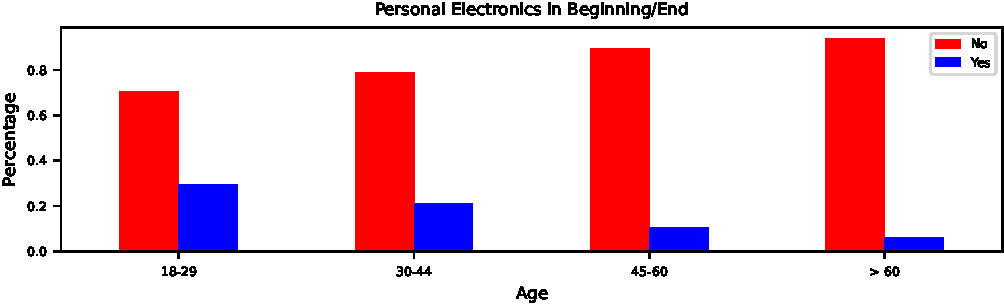
\includegraphics{hypo_1.pdf} % note no [width=\textwidth] needed
%    \caption{This is a figure that spans the page.}
%\end{figure}

\bibliography{bibliography}
\bibliographystyle{icml2023}

\end{document}


% This document was modified from the file originally made available by
% Pat Langley and Andrea Danyluk for ICML-2K. This version was created
% by Iain Murray in 2018, and modified by Alexandre Bouchard in
% 2019 and 2021 and by Csaba Szepesvari, Gang Niu and Sivan Sabato in 2022.
% Modified again in 2023 by Sivan Sabato and Jonathan Scarlett.
% Previous contributors include Dan Roy, Lise Getoor and Tobias
% Scheffer, which was slightly modified from the 2010 version by
% Thorsten Joachims & Johannes Fuernkranz, slightly modified from the
% 2009 version by Kiri Wagstaff and Sam Roweis's 2008 version, which is
% slightly modified from Prasad Tadepalli's 2007 version which is a
% lightly changed version of the previous year's version by Andrew
% Moore, which was in turn edited from those of Kristian Kersting and
% Codrina Lauth. Alex Smola contributed to the algorithmic style files.
